\chapter{Basic Formatting}
This chapter will show basic formatting of text, figures, tables and equations. It will also be mostly filled with `dummy' text so there is something to look at.

\section{Body Text}
Body text has a $1/2$ inch indent on all paragraphs and double spaced lines.
\lipsum[6]
\section{Figures, In-Text Citations, and Footnotes}
Figure~\ref{fig:athletic logo} is an example of how images can be formatted. Additionally, citations to references will be shown such \cite{latexcompanion}. Footnotes\footnote{This is a footnote text message that doesn't offer much information.} will behave like this\footnote{This is another footnote.}.

\begin{figure}[!ht]
	\centering
	\footnotesize
	
\includegraphics[width=2in]{athletic-bw.png}
	\caption{An Athletic logo?}
	\label{fig:athletic logo}
\end{figure}\vspace{-1em} % can be useful to pull following text closer... sometimes, other times messes up format.

A larger graphic example is shown on Page~\pageref{fig:ramp test 1} as Figure~\ref{fig:ramp test 1}. \lipsum[8] 

\begin{figure}[!ht]
	\centering
	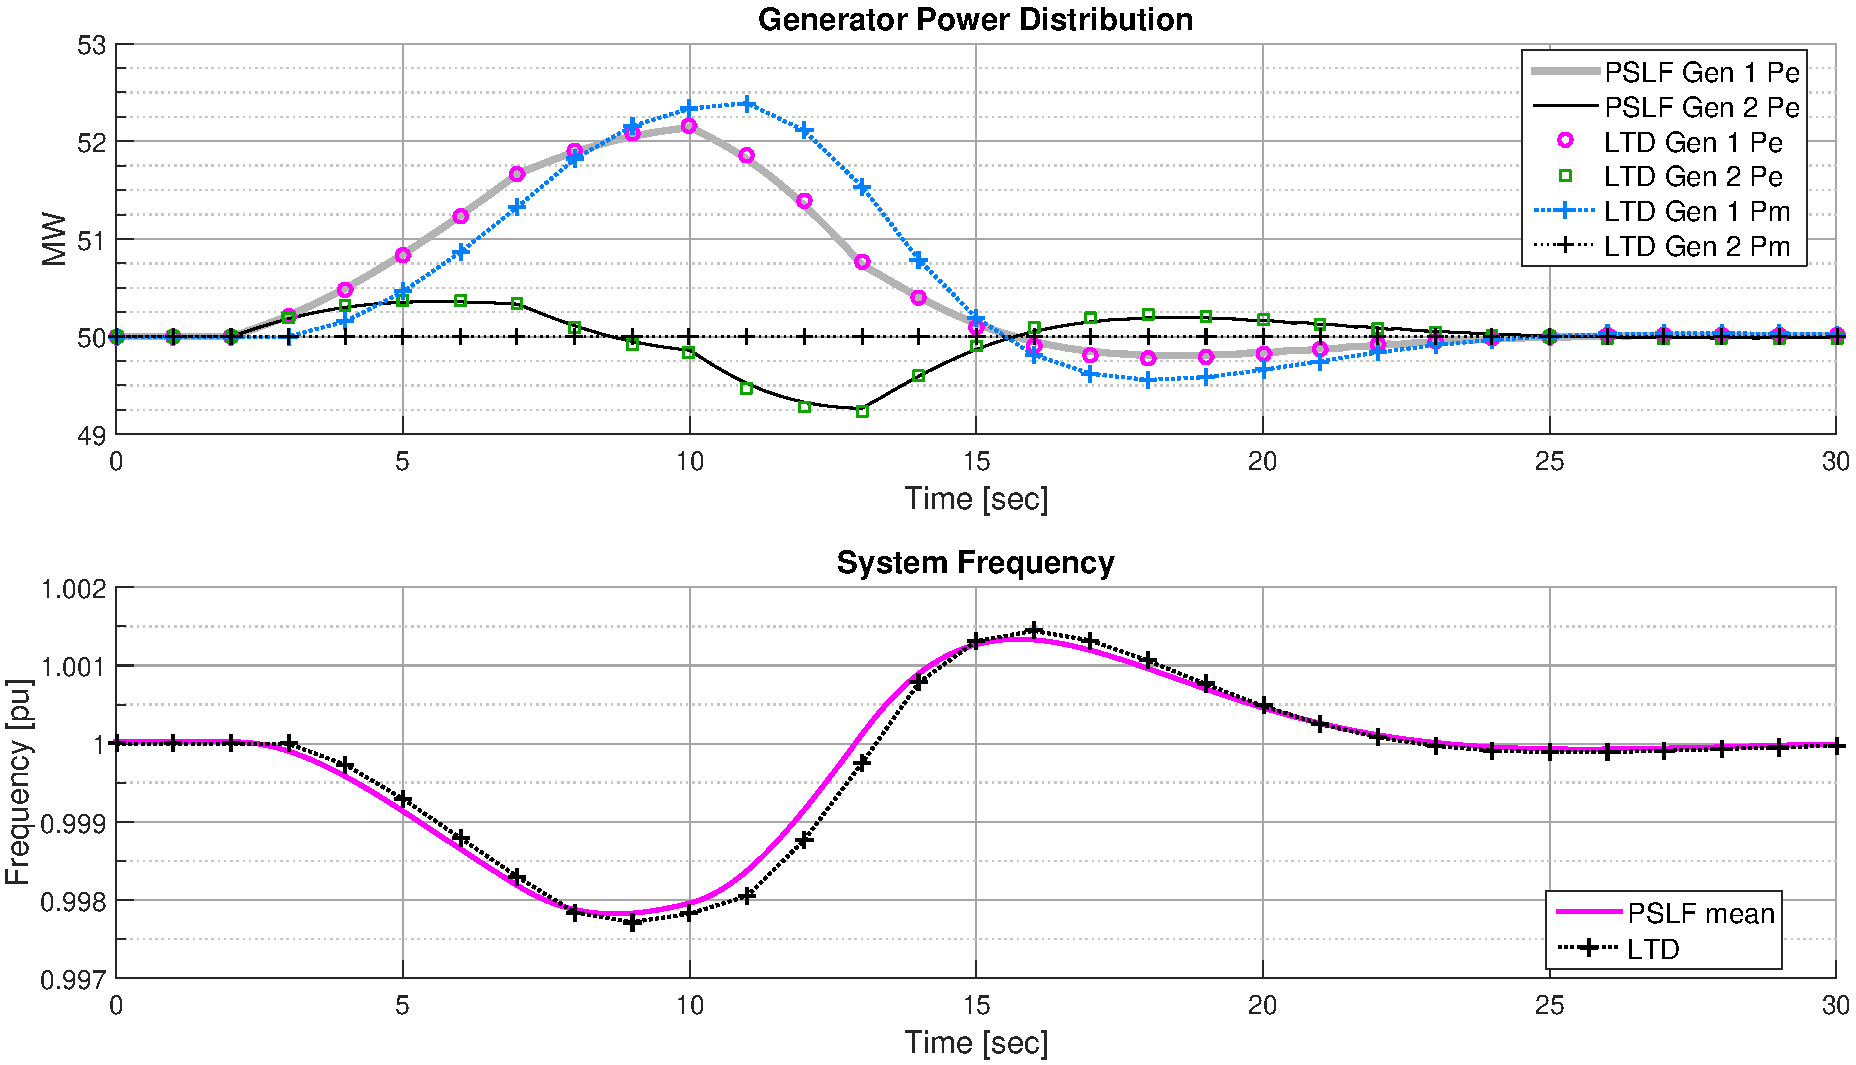
\includegraphics[width=\linewidth]{test/ramp1sec.pdf}
	\caption[60 Second Ramp Test.]{This is a fairly large graphic but can easily be set to any desired width. Additionally, this is a super long caption that would break the table of contents formatting if it weren't for an optional `short title' parameter. There's even a citation in here\cite{stajcar}.}
	\label{fig:ramp test 1}
\end{figure}%\vspace{-1em}

\lipsum[15]

\section{Equations}
	A somewhat fancy equation involving symbols and an integral is pretty easy to put together. \lipsum[5] %
	\begin{equation}{\label{eq:ssSoln}}
		x(t) = \Phi(t) x(0) + \int_{0}^{t}\Phi(t-\tau)Bu(\tau) \text{d}\tau.
	\end{equation}\eqcaption{An example of optional equation captions}

	\lipsum[6]\ Unlike Equation~\ref{eq:ssSoln}, Equation~\ref{eq:one} is pretty basic.%
	\begin{equation}{\label{eq:one}}
		a+b=c
	\end{equation}\eqcaption{.}
	
	Aligned rows of equations are also possible using the \verb|align*| environment and a custom \verb|numberthis| command. The following math is very math.
	\begin{align*}
		G(\$) &= \dfrac{20}{\$(\$+5)(\$+10)}\\
		\zeta = 0.59116 &, \Phi_M = 58.59\\
		\therefore \omega_{\Phi_M} &= \omega \angle -121.41^\circ\\
		\text{From Bode: } \omega_{\Phi_M} &= 1.9 \\
		\abs{\omega_{\Phi_M}} &= -14.3 \\
		\therefore K &= 10^\frac{14.3}{20} =5.188 \text{ abs} \numberthis \label{eq:align}
	\end{align*}\eqcaption{Some Gain Calculation}

\section{Tables}
Tables can look like Table~\ref{tab:exp1}. Notice the slimming effect of no vertical lines\ldots .
 Quisque vehicula, urna sed
ultricies auctor, pede lorem egestas dui, et convallis elit erat sed nulla. Donec luctus. 

\begin{table}[h]
	\centering
	\begin{tabular}{@{} l r r r r @{}} 	
		\toprule % @ signs to remove extra L R space
		\footnotesize % this will make the table font 10pt
		& \multicolumn{1}{c}{Experiment 1}	& \multicolumn{1}{c}{Experiment 2}	& \multicolumn{1}{c}{Experiment 3}	& \multicolumn{1}{c}{Experiment 4} \\
		\midrule
		Old	& 29.631	& 17.333	& 222.999	& 11.222 \\
		Not Old	& 54.321	& 166.233	& 556.123	& 54.666 \\
		Almost New	& 118.791 &	54.289 &	445.321 &	88.122 \\
		New& 	222.897	& 10.000 &	777.000	 & 90.100 \\
		\bottomrule
	\end{tabular}
	\caption{An example table with no vertical lines.}
	\label{tab:exp1}
\end{table}

Table style may be altered to a slightly different style if it seems appropriate.  Quisque vehicula, urna sed
ultricies auctor, pede lorem egestas dui, et convallis elit erat sed nulla. Donec luctus. 
Notice that chapters start on a new page.
